\section{Data Flow in SOC}

The first step of the process is to pull in logs and telemetry from a variety of security monitors (NDR, WAF, and UEBA). Each of the monitoring tools consistently monitors an aspect of the organization infrastructure and makes its relevant telemetry information available to the SOC:

\begin{itemize}[itemsep=0pt,parsep=0pt,topsep=0pt,partopsep=0pt]
    \item \textbf{NDR (Network Detection and Response)}: These systems monitor all directions of network traffic in and across the organization. They assist in recognizing unusual or suspicious activities, such as advanced attacks or movement of threats from one system to another system in the network.
    \item \textbf{WAF (Web Application Firewall)}: These systems monitor HTTP traffic and provide filtering and monitoring protection to web applications and services. These systems will be able to proactively block known attacks, such as SQL injections, XSS, and unauthorized access attempts.
    \item \textbf{UEBA (User and Entity Behavior Analytics)}: These systems build user behaviors models and machine learning around baseline activity and analysis deviations from that baseline. These systems assist in recognizing insider threats, compromised accounts, and privilege escalation.
\end{itemize}

\begin{figure}[H]
    \centering
    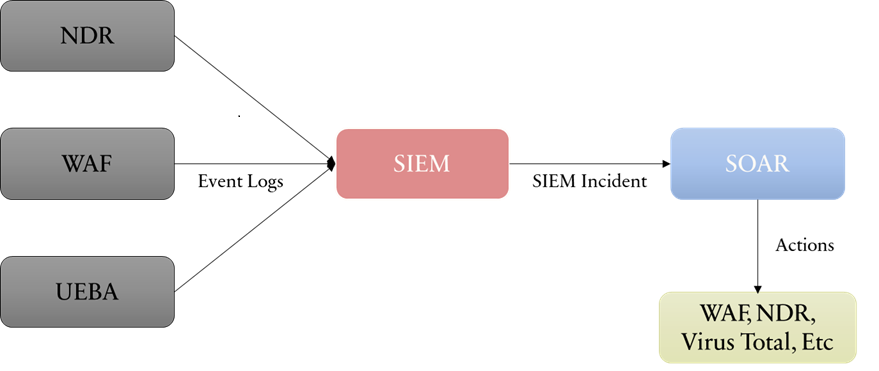
\includegraphics[width=0.9\linewidth]{images/data_flow_soc.png}
    \caption{Data Flow in Security Operations Center (SOC)}
    \label{fig:data-flow-soc}
\end{figure}

All the data collected from these systems is funneled into the Security Information and Event Management (SIEM) system. SIEM is responsible for log aggregation, normalization of event data, correlation of security events, and threat detection and identification of potentially significant incidents. The SIEM will use correlation rules and heuristics to generate alerts for suspicious suspicious behavior and known indicators of compromise. The SIEM provides one central visibility/detection hub for the SOC. 

The alerts, along with the enhanced context in the SIEM, is forwarded to the Security Orchestration, Automation, and Response (SOAR) system:

\begin{itemize}[itemsep=0pt,parsep=0pt,topsep=0pt,partopsep=0pt]
    \item \textbf{SOAR}: Automating the triage and response process through playback and workflows. Orchestrating actions that happen through tools, enhancing (ex. IP reputation check), or taking action (ex. automated or manned response).
\end{itemize}

The SOAR may interface with tools when taking action or during the enrichment process:

\begin{itemize}[itemsep=0pt,parsep=0pt,topsep=0pt,partopsep=0pt]
    \item \textbf{Threat Intelligence (e.g., VirusTotal)}: Provides context for IP, domains, file hashes, and URLs to leverage for detection and validation of alerts.
    \item \textbf{Internal Tools (e.g., WAF, NDR)}: These tools can be part of automated response to isolate endpoints, block malicious traffic or escalate incidents.
\end{itemize}

Finally, the SOAR platform creates a structured response which could consist of a series of automated actions and manual decisions by analysts. All this will be recorded in such a way that the full flow from data collection through response would be tracked to help with auditing, compliance, and continuous improvement of SOC activities.

\section{Security Information and Event Management (SIEM) in SOC}

A key part of any SOC (Security Operations Center) is the organization’s Security Information and Event Management (SIEM) which allows for data aggregation and correlation as part of the monitoring of cybersecurity. SIEM systems aggregate event and log data from all areas of an organization’s digital infrastructure (such as endpoints, servers, network devices, firewalls, intrusion detection systems, cloud infrastructure, and applications) and evaluate the data as a whole. The goal of a typical SIEM is to aggregate all the organization's relevant security logs into a system that allows it to determine the current state of security and to provide real-time visibility into potential security incidents. A SIEM can receive data from lots of different sources, normalize the data, apply correlation rules to the data, and generate alerts for SOC analysts to prioritize and investigate. Microsoft, ~\cite{microsoftsiem}, explains that SIEM solutions were developed primarily to help security teams deal with evolving cyberattacks sooner, enabling them to get ahead of a potentially damaging incident or intrusion and to remain compliant with regulations, by keeping detailed audit records and forensic information.

In a traditional SOC operational model, SIEM is the initial source of alert generation, so SIEM uses it own correlation rules, statistical models, and sometimes machine learning, to detect anomalies such as unusual user behavior, suspicious login patterns, and known indicators of compromise (IoCs). Alerts are triaged by analysts to determine whether they are true threats or false positives.  The leading SIEMtools (e.g., IBMQRadar, SplunkEnterprise Security, Microsoft Sentinel, ArcSight) generally provide customizable dashboards, threat detection use-cases, and compliant reporting together making them a great fit for enterprise and government cybersecurity needs.

Understanding the distinction between a SIEM and a SOAR is an important differentiator since both will be used in a SOC. SIEM is focused on data collection, aggregation, and detection. SOAR offers response orchestration, automation, and execution of the workflows. SIEM is passive in that it tells security teams about potential incidents; SOAR is active in that it can automatically take defined actions, including but not limited to blocking the IP, sending out notifications, or following a playbook, based on the data SIEM collected and aggregated. As noted by Palo Alto Networks~\cite{paloalto}, SIEM can answer “what happened?” or “where did it happen?”; whereas SOAR can answer “what do we do about it?”

Moreover, SIEM solutions, especially new-age SIEMs, tend to operate at a much higher volume of data, integrating with multiple systems and ingesting terabytes of log data daily. This data-centric approach has made SIEMs very strong for long-term log retention and forensic investigations, especially for companies that have regulatory obligations to preserve logs. On the other hand, SIEMs can be challenged by alert fatigue, false positives, and unnecessary investigation, all of which can be mitigated by combining the SIEM capabilities with SOAR capabilities to automate triaging, enrichment, and decision-making activities. As Gartner mentions, they recommend modern SOCs do not think of SIEM and SOAR as disparate or competing solutions, but rather as systems that, when combined, will enhance the efficiency and responsiveness of all cybersecurity operations~\cite{gartner-siem-soar}.

In conclusion, SIEM is the eyes and ears of the SOC as it offers centralized, real-time capture of security relevant events occurring within a wide variety of digital assets as it relates to the industry landscape. When SIEM collects and correlates the relevant data and the data is ingested by SOAR, the action can be scaled, automated, and driven by intelligence. In defense and national critical infrastructure, SIEM is the detection tool and SOAR is the orchestration tool. Together they form the core ability for effective cyber defense and incident response in a SOC. The combination of SIEM and SOAR is a powerful force multiplier for SOCs, enabling them to operate at scale, with speed, and with intelligence. The effectiveness of this combination is evident in the way it reduces the Mean Time to Detect (MTTD) and Mean Time to Respond (MTTR) to security incidents, which are critical metrics for any SOC.

\begin{table}[H]
\centering
\caption{Comparison of SIEM and SOAR in SOC}
\begin{tabular}{|p{4cm}|p{5cm}|p{5cm}|}
\hline
\textbf{Feature} & \textbf{SIEM (Security Information and Event Management)} & \textbf{SOAR (Security Orchestration, Automation, and Response)} \\
\hline
Primary Function & Aggregates and correlates log data for threat detection & Automates response actions and orchestrates tools \\
\hline
Focus Area & Monitoring, alerting, and data analysis & Incident response, workflow automation, playbook execution \\
\hline
Data Sources & Logs from endpoints, servers, network devices, and applications & Inputs from SIEM, threat intel feeds, manual triggers \\
\hline
Response Capability & Alert generation only (manual response required) & Supports automated and manual responses \\
\hline
Typical Output & Dashboards, correlation alerts, compliance reports & Executed actions, response workflows, status tracking \\
\hline
Alert Handling & Detects and prioritizes alerts; triage is manual & Automates triage, enrichment, and routing \\
\hline
Challenges Addressed & Data visibility, compliance, threat correlation & Alert fatigue, response delays, process inconsistency \\
\hline
\end{tabular}
\label{tab:siem-vs-soar}
\end{table}

\section{SIEM Incident Flow to SOAR}

One of the most integral integrations with a Security Operations Center (SOC) is that of SIEM and the SOAR platform. The integration allows for the easy transition from threat detection (by a SIEM system) to response (orchestration provided by SOAR). A SIEM incident is typically an event or an alert that has been generated based on the event correlations of log data received from different security tools, e.g., firewall, endpoint protection software, network devices, servers, and cloud environments. As stated by Microsoft~\cite{microsoftsiem}, the SIEM looks for known attack patterns, anomalies, and user behavior based on correlation rules or machine learning models, as it continuously collects and analyzes the data from multiple sources. Once a SIEM flag has been raised for an event, it is then seen as an incident along with a complete set of metadata attached to the incident.

A typical SIEM incident contains structured fields such as:

\begin{itemize}[itemsep=0pt,parsep=0pt,topsep=0pt,partopsep=0pt]
    \item \textbf{Alert ID}: Unique identifier for the incident or alert.
    \item \textbf{Timestamp}: Time at which the event occurred or was detected.
    \item \textbf{Source IP / Host}: Origin of the suspicious activity.
    \item \textbf{Destination IP / Host}: Targeted system or service.
    \item \textbf{Username}: Account associated with the event (if applicable).
    \item \textbf{Severity Level}: Assigned severity (e.g., low, medium, high, critical).
    \item \textbf{Event Type / Rule Name}: Category or rule that triggered the alert (e.g., brute force, malware, lateral movement).
    \item \textbf{Raw Logs / Correlation Data}: Detailed evidence or event logs that support the detection.
    \item \textbf{Tactic / Technique (if mapped)}: MITRE ATT\&CK classification, if supported.
\end{itemize}

This incident data is then sent in real-time or near real-time to the Security Orchestration, Automation, and Response (SOAR) platform via APIs, message queues, or webhooks. As noted by Palo Alto Networks~\cite{paloalto}, the SOAR platform provides full incident details so that it can is quickly enriched, triaged and acted upon.

Upon receipt of the incident, the SOAR system begins triaging the incident. It might apply severity filters, check asset criticality, or leverage external threat intelligence repositories (e.g., VirusTotal, AbuseIPDB) to enrich incident data. Based on this context, the SOAR platform implements action playbooks. Actions could include:

\begin{itemize}[itemsep=0pt,parsep=0pt,topsep=0pt,partopsep=0pt]
    \item Notification of an analyst or team
    \item Suspending access from the user's IP address using a Fiewall or an EDR
    \item Isolate host from the network
    \item Ask for additional context from the threat feeds or a SIEM
    \item Resolve automatically if shown to be a known benign pattern.
\end{itemize}

During this process, the SOAR platform stores a case file with the timeline of actions, analyst comments and responses. This automation enhances consistency and greatly reduces the Mean Time to Respond (MTTR), particularly important at scale in a SOC, according to Gartner~\cite{gartner-siem-soar}.

Therefore, the SIEM-to-SOAR pipeline allows SOCs to transform raw detections into intelligent, actionable response, allowing for operational oversight and auditability.
